\chapter{CUDA\label{cap:cuda}}

CUDA (\textit{Compute Unified Device Architecture}) é a arquitetura de computação paralela da NVIDIA para GPUs (\textit{Graphic Processor Unit} - Unidade de Processamento Gráfico). Graças à combinação de CPUs multinúcleo com as GPUs, os PCs e \textit{laptops} entraram na era da computação na teraescala \cite{Kirk2010}, abrindo a possibilidade para pesquisadores e empresas de diversas áreas tomarem proveito da computação de alto desempenho. Muitos produtos comerciais já são compatíveis com CUDA, como o Mathematica e o MatLab.
	
	A principal diferença na comparação com a CPU é o fato da GPU ser especializada em computação intensiva (ponto flutuante) e paralela - historicamente necessárias para reinderização de imagens \cite{CUDACpg}. Do ponto de vista do \textit{hardware}, a GPU utiliza mais transistores para operações matemáticas (figura \ref{figCPU_GPU}). 
	
	\begin{figure}[hpt]
		\begin{center}
			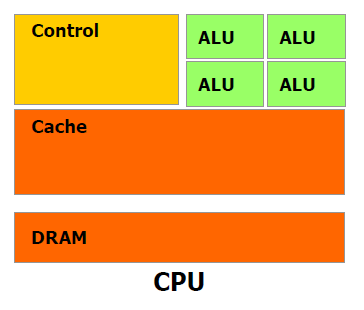
\includegraphics[width=6cm]{figs/cuda/CPU-Transistores.png}
			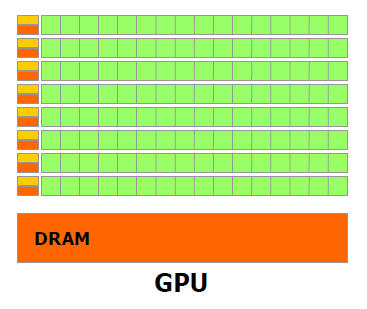
\includegraphics[width=6cm]{figs/cuda/GPU-Transistores.png}
		\end{center}
		\caption{\label{figCPU_GPU}Representação esquemática da utilização de transistores na CPU e na GPU. Note que o número de transistores dedicados às operações matemáticas é muito superior, enquanto o controle de fluxo de dados e a memória \textit{cache} estão naturalmente paralelizados. Retirado de \cite{CUDACpg}.}
	\end{figure}

	No modelo híbrido de programação, parte do código é executada na CPU, parte na GPU. A porção executada na placa de vídeo deve possuir características para tirar proveito da arquitetura CUDA, ou seja, ser paralelizável e necessitar de cálculo intensivo. 
	
	Para programar uma GPU compatível com CUDA utiliza-se o CUDA C, uma extensão do ANSI C disponibilizada gratuitamente pela NVIDIA. A CPU (\textit{host}) executa o código de maneira sequencial, enquanto a GPU (\textit{devide}) utiliza o conceito de \textit{Multithreading} para a computação paralela. Ou seja, na arquitetura CUDA, a CPU e a GPU são complementares.
	
	Na figura \ref{figCodigo} há um exemplo. O objetivo do programa é somar dois vetores, tarefa que pode ser facilmente paralelizada pois a soma de cada elemento acontece de maneira independente. No início do código uma função chamada \texttt{VecAdd} é declarada. Seus parâmetros são três ponteiros para um número real e, no corpo da função, acontece a soma dos elementos do vetor:
	
	\begin{equation}
		C[i] = A[i] + B[i]
	\end{equation}

\begin{figure}[hpt]
		\begin{center}
			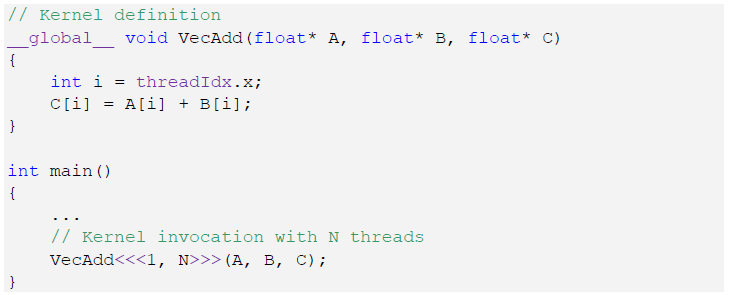
\includegraphics[width=12cm]{figs/cuda/ExemploCodigo.png}
		\end{center}
		\caption{\label{figCodigo}. Exemplo de código em CUDA C. A função \texttt{VecAdd} adiciona dois vetores $A$ e $B$ de ordem $N$ e armazena o resultado no vetor $C$. Retirado de \cite{CUDACpg}.}
	\end{figure}

	Naturalmente sente-se falta de um \textit{loop} percorrendo todos os $N$ elementos do vetor. Porém, dentro do CUDA C, esse \textit{loop} é substituído por \mbox{\texttt{int i = threadIdx.x}}, indicando que, agora, há uma \textit{thread} dedicada à soma de cada um dos $i$ elementos.
	
	Entretando, dentro da função \texttt{VecAdd()} não há referência ao tamanho dos vetores sendo somados. Então, como \texttt{VecAdd()} sabe que precisa de $N$ \textit{threads} para executar a soma de todos os $N$ elementos em paralelo? Essa informação está contida na chamada da função \texttt{VecAdd()} dentro da \texttt{main()}. A sintaxe \texttt{<<<1, N>>>} diz ao compilador que a função precisará de $1$ bloco com $N$ \textit{threads}/bloco. Se for necessário lidar com um vetor maior, basta solicitar mais \textit{threads}, o que exige o conhecimento da arquitetura CUDA. A cláusula \texttt{\_\_\_global\_\_\_} na definição de \texttt{VecAdd()} indica que essa função será executada na GPU.

	\begin{figure}[hpt]
		\begin{center}
			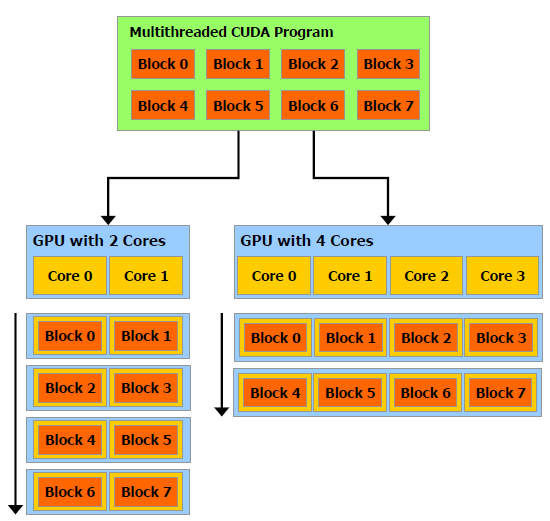
\includegraphics[height=6cm]{figs/cuda/Blocos_nas_CPUs.png}
			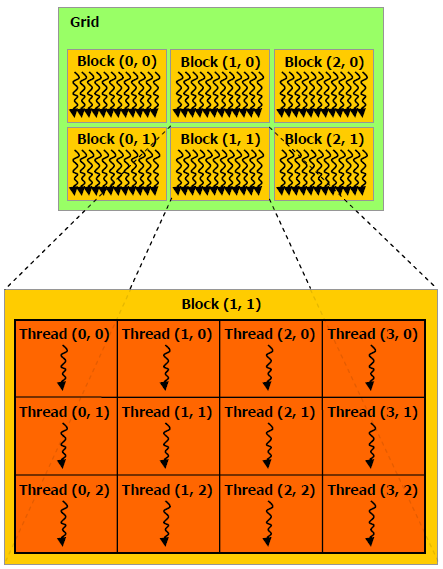
\includegraphics[height=6cm]{figs/cuda/Blocos_No_Grid_E_Suas_threads.png}
		\end{center}
		\caption{\label{figHierarquiaThreads}Estrutura hierárquica das \textit{threads}. No lado esquerdo há uma representação da distribuição de blocos entre os núcleos. Esse processo, que é automático, permite a construção de programas altamente escaláveis. À direita está a disposição das \textit{threads} dentro dos blocos. Retirado de \cite{CUDACpg}.}
	\end{figure}

	O número de \textit{threads} por bloco é uma característica de cada placa, e pode ser obtido em tempo de execução. Cada núcleo de processamento executa um bloco com suas $N$ \textit{threads}/bloco. Caso o número necessário de \textit{threads} exija mais blocos do que os núcleos disponíveis, os blocos são distribuídos automaticamente pela CUDA (figura \ref{figHierarquiaThreads}), tornando esse processo transparente para o programador.
	
	Essa facilidade permite escrever códigos altamente escaláveis. Nota-se na figura \ref{figHierarquiaThreads} que um mesmo programa pode rodar em placas simples, com poucos núcleos, ou nas mais sofisticadas com centenas de núcleos. Isso vale também para a utilização de mais de uma placa.